\documentclass[a4paper, 11pt]{article}
\usepackage[T2A]{fontenc}
\usepackage[utf8]{inputenc}
\usepackage[russian]{babel}
\usepackage{indentfirst}
\usepackage{amssymb}
\usepackage{enumitem}
\usepackage{hyperref}
\usepackage{geometry}
\usepackage{mathtools}
\usepackage{setspace}
\usepackage{amsmath,amsfonts,amssymb,amsthm,mathtools}
\usepackage{tikz}
\usepackage{tikzsymbols}
\usepackage{soul}
\geometry{a4paper,top=2cm,bottom=2cm,left=2cm,right=2cm}

\usepackage{fancyhdr}
\pagestyle{fancy}

\makeatletter
\def\thickhrulefill#1{\leavevmode\leaders\hrule height#1\hfill\kern\z@}
\makeatother

\usepackage{mathtools}
\DeclarePairedDelimiter\ceil{\lceil}{\rceil}
\DeclarePairedDelimiter\floor{\lfloor}{\rfloor}

% Розовый текст в рамке
\newcommand{\pinkframed}[2][rectangle,draw,fill=purple!20]{%
	\tikz[baseline=-0.6ex] \node [#1]{#2};}%

\newenvironment{result} { \sgap
	\smallskip
	\pinkframed{ \textbf{Ответ:} }}{}

\renewcommand{\headrule}{
	\color{black}\vspace{-8pt}
	\thickhrulefill{.6pt}

	\vspace{-9pt}\thickhrulefill{2.4pt}
}

\newcommand{\un}{\underline}
\newcommand{\ov}{\overline}


\newcommand{\NN}{\mathbb{N}}
\newcommand{\ZZ}{\mathbb{Z}}
\newcommand{\RR}{\mathbb{R}}
\newcommand{\QQ}{\mathbb{Q}}
\newcommand{\CC}{\mathbb{C}}

\newcommand{\A}{\; \forall \;}
\newcommand{\E}{\; \exists \;}
\newcommand{\nE}{\; \nexists \;}

\newcommand{\vp}{\varphi}
\newcommand{\e}{\varepsilon}
\newcommand{\lm}{\lambda}
\newcommand{\ds}{\displaystyle}

\newcommand{\prob}[1]{\item \textbf{(#1 баллов)}.}


\rhead{Парфенов Артем БПМИ219}
\lhead{Основы матричных вычислений ДЗ-1}
\begin{document}

	\subsection*{Задачи по лекции 1}
	\begin{enumerate}
		\prob{11} Пусть задан вектор $u\in\mathbb{C}^n\colon \|u\|_2=1$. Найдите все $\alpha \in \mathbb{C}$, для которых $A = I - \alpha u u^*$ является: 1) эрмитовой 2) косоэрмитовой 3) унитарной 4) нормальной. Для пункта 3) также нарисуйте найденные $\alpha$ на комплексной плоскости.
		
		\begin{enumerate}
			\item $A = I - \alpha u u^* = A^*$ 
			
				$\begin{pmatrix}
					1 - \alpha |u_1|^2 && \alpha u_1 u_2^*  && \dots \\
					\alpha u_1^* u_2 && 1 - \alpha |u_2|^2   && \dots \\
					\vdots  && \vdots && \vdots \\
				\end{pmatrix}$
			
				Если сопрячь $ \alpha u_1 u_2^*$, получится $\alpha u_1^* u_2$
				
				Эрмитово сопряжение это транспонирование(которое сейчас просто отразит элементы относительно диагонали) и сопряжение, как я показал. 
				
				Тогда получается, что 
				
				$\begin{pmatrix}
					1 - \alpha |u_1|^2 && \alpha u_1 u_2^*  && \dots \\
					\alpha u_1^* u_2 && 1 - \alpha |u_2|^2   && \dots \\
					\vdots  && \vdots && \vdots \\
				\end{pmatrix}^* = $ $\begin{pmatrix}
				1 - \alpha^* |u_1|^2 && \alpha^* u_1^* u_2  && \dots \\
				\alpha^* u_1 u_2^* && 1 - \alpha^* |u_2|^2   && \dots \\
				\vdots  && \vdots && \vdots \\
			\end{pmatrix}$
		
			равенство выполняется $\Longleftrightarrow \alpha^* = \alpha$
			
			Для скаляра имею в виду под звездочкой комплексное сопряжение.
			
			\item $A = I - \alpha u u^* = -A^*$
			
			$\begin{pmatrix}
				1 - \alpha |u_1|^2 && \alpha u_1 u_2^*  && \dots \\
				\alpha u_1^* u_2 && 1 - \alpha |u_2|^2   && \dots \\
				\vdots  && \vdots && \vdots \\
			\end{pmatrix}^* = $ $\begin{pmatrix}
				-1 + \alpha^* |u_1|^2 && -\alpha^* u_1^* u_2  && \dots \\
				-\alpha^* u_1 u_2^* && -1 + \alpha^* |u_2|^2   && \dots \\
				\vdots  && \vdots && \vdots \\
			\end{pmatrix}$
		
			Значит 
		
			$\begin{cases}
				\alpha = -\alpha^* \\
				2  = \alpha^* |u_1|^2 + \alpha |u_1|^2 \\
			\end{cases}$
		
			$\sqsupset \alpha = a + ib \implies a + ib = -a + ib \Longleftrightarrow \alpha = ib$ - первое условие
			
			$2 = -ib |u_1|^2 + ib|u_1|^2 \Longleftrightarrow 2 = 0$(юзаю результат первого уравнения, что у альфы только мнимая часть)
			
			получается, что такого не бывает.
			
			
			\item $A = (I - \alpha u u^*) \cdot (A^*) = I$
			
			$(I - \alpha u u^*) \cdot (I - \alpha u u^*)^* = I$
			
			$(I - \alpha u u^*) \cdot (I^* - \alpha^* u u^*) = I$
			
			$I - I \alpha^* u u^* - I \alpha u u^* + ( \alpha u u^*) \cdot (\alpha^* u u^*) = I$
			
			$I - \alpha^* u u^* - \alpha u u^* + ( \alpha u u^*) \cdot (\alpha^* u u^*) = I$
			
			$\alpha^* u u^* + \alpha u u^* = ( \alpha u u^*) \cdot (\alpha^* u u^*)$
			
			$\alpha^* u u^* + \alpha u u^* =  |\alpha|^2  \cdot (u u^* u u^*)$
			
			$u^* u = 1$ по условию единичности нормы.
			
			$\alpha^* u u^* + \alpha u u^* =  |\alpha|^2  u u^*$
			
			$(\alpha + \alpha^*) uu^* = |\alpha|^2  u u^*$
			
			$(\alpha + \alpha^*) = |\alpha|^2 \xleftrightarrow{\alpha = a + bi}  2a = a^2 + b^2$
			
			Ответ: выполняется при альфах, для которых верно равенство выше и см. рисунок.
						
			\bigskip
			
			Рисунок:
			
			\begin{figure}[h]
				\center{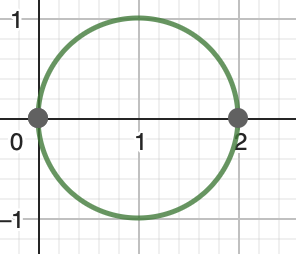
\includegraphics[scale=1.0]{1-3.jpg}}
				\caption{Вертикальная ось - мнимая часть.}
			\end{figure}
		
		\newpage
		
		\item $(I - \alpha u u^*) \cdot (A^*) = A^* \cdot (I - \alpha u u^*)$
		
			$(I - \alpha u u^*) \cdot (I^* - \alpha^* u u^*) = (I^* - \alpha^* u u^*) \cdot (I - \alpha u u^*)$
			
			$I - \alpha^* u u^* - \alpha u u^* + ( \alpha u u^*) \cdot (\alpha^* u u^*) = I - \alpha u u^* - \alpha^* u u^* + |\alpha|^2 u u^*$
			
			$|\alpha|^2 u u^* = |\alpha|^2 u u^* \Longleftrightarrow \alpha \in \CC$
								
		\end{enumerate}
		
		
		
		\prob{11} Пусть $e = (1,1,1)^\top$ и $e_1 = (1,0, 0)^\top$. Найдите $\|A\|_{2023}$, где $A = ee_1^\top$.
		
			$A = \begin{pmatrix}
				1 && 0 && 0 \\ 
				1 && 0 && 0 \\
				1 && 0 && 0 \\
			\end{pmatrix}$
		
			$\|A\|_{2023} = \sup_{x \neq 0} \frac{\|Ax\|_{2023}}{\|x\|_{2023}} = \sup_{\|t\|_{2023}  = 1} \|At\|_{2023}$	
			
			$\|t\|_{2023} = (|t_1|^{2023} + |t_2|^{2023} + |t_3|^{2023})^{\frac{1}{2023}} = 1$
			
			$|t_1|^{2023} + |t_2|^{2023} + |t_3|^{2023} = 1$ значит каждая координата не больше единицы.
			
			$At = (t_1, t_1, t_1)$ норма максимальная при $t_1 = 1$ 
			
			$\sup_{\|t\|_{2023}  = 1} \|At\|_{2023}$ уже векторная норма потому 
			
			$\sup_{\|t\|_{2023}  = 1} \|At\|_{2023} = \sqrt[2023]{1^{2023} + 1^{2023} + 1^{2023}} = \sqrt[2023]{3}$
		
		
		
		\prob{12}
		\begin{enumerate}
			\item Докажите, что 
			\[
			\|x\|_2 \leq \|x\|_1 \leq \sqrt{n} \|x\|_2 \quad \forall
			x\in\mathbb{C}^n.
			\]
			На каких векторах $x$ достигаются равенства?
			
				\begin{enumerate}
					\item $\|x\|_2 \leq \|x\|_1$
						
						$\displaystyle \|x\|_2 = \sqrt{\sum_{i = 1}^{n} |x_i^2|} \leqslant \sqrt{\sum_{i = 1}^{n} |x_i^2| + 2 \sum_{i \neq j} |x_i||x_j|} = \| x \|_1$
						
						Под корнями стоит одна и та же сумма, но в первой норме мы еще прибавили что-то неотрицательное, потому все верно.
						
					\item $\|x\|_1 \leq \sqrt{n} \|x\|_2$
					
							\medskip
					
						$\displaystyle \| x\|_1 = \frac{\displaystyle \sum_{i} |x_i|}{n}] \leqslant \| x \|_2 = \sqrt{\frac{\displaystyle \sum_i |x_i|^2}{n}}$
						
						если вынести справа из под корня n получится в точности то, что в условии, а выполняется оно в силу неравенства о среднем.
						
						
				\end{enumerate}
			
			Точно достигается на нулевых. Левое помимо этого, когда одна из коодинат вектора единичка, а остальные - нули(удвоенные произведения равны нулю будут).
			
			Правая часть помимо нулевых еще на векторах, пропорциональных единичному.			
			
			\item Используя неравенство из (а), покажите, что
			\[
			\frac{1}{\sqrt{n}} \|A\|_2 \leq  \|A\|_{1} \leq \sqrt{m} \|A\|_2 \quad \forall A\in\mathbb{C}^{m\times n}.
			\]
			
			$\square$
			
					\begin{enumerate}
						\item $\frac{1}{\sqrt{n}} \|A\|_2 \leq  \|A\|_{1}$
						
							Распишем по определению:
							
								$\frac{1}{\sqrt{n}} \|A\|_2 = \sup_{x \neq 0} \frac{\| Ax\_2|}{\sqrt{n} \| x \|_2} \leqslant $
								
								вспомним результат предыдущего пункта и заменим в знаменателе вторую норму на первую. Также можно сделать в числителе не испортив знака неравенства.
								
								$\leqslant \sup_{x \neq 0} \frac{\| Ax \|_1}{\| x \|_1 } $ а это как раз первая норма - успех
								
						\item $\|A\|_{1} \leq \sqrt{m} \|A\|_2$
						
							снова определение первой нормы и меняем первую на вторую
							
							$\| Ax \|_1 \leqslant \sup_{x \neq 0} \frac{\| Ax \|_1}{\| x \|_2} \leqslant$ теперь домножим на корень, чтобы подогнать в числителе ко второй норме
							
							$\leqslant \sup_{x \neq 0} \sqrt{m} \frac{\| Ax \|_2}{\| x \|_2} $ а это как раз вторая норма домноженная на корень из м
							
						$\hfill \blacksquare$
						
					\end{enumerate}
			
				
		\end{enumerate}
		\prob{16} 
		Обозначим $A = \begin{bmatrix}0 & 1 \\ 0 & 0 \end{bmatrix}$ и $A_n = \begin{bmatrix} 0 & 1 \\ 1/n & 0 \end{bmatrix}, n\in\mathbb{N}$.
		\begin{enumerate}
			\item Обоснуйте сходимость $A_n\to A$, $n\to\infty$.
				
				$\|A_n - A\|_F = \|\begin{pmatrix}
					0 && 0 \\
					\frac{1}{n} && 0 \\
				\end{pmatrix}\|_F = \sqrt{\frac{1}{n^2}} \to 0$  при $n \to +\infty$ значит есть сходимость.
			
			\item Найдите собственные разложения $A_n = S_n \Lambda_n S_n^{-1}$ и проверьте существование пределов для каждой из $S_n$,$\Lambda_n$ и $S_n^{-1}$. Почему не у всех из этих матриц существует предел?
			
				Ищем харчлен:
				
				$det \begin{pmatrix}
					-\lambda && 1 \\
					\frac{1}{n} && -\lambda \\
				\end{pmatrix}$
			
				$\lambda^2 - \frac{1}{n} = 0 \Longleftrightarrow \lambda = \pm \frac{1}{\sqrt{n}}$
				
				$\begin{pmatrix}
					-\frac{1}{n} \ && 1 \\
					\frac{1}{n} && -\frac{1}{n} \\
				\end{pmatrix} \rightsquigarrow{\textit{УСВ}} \begin{pmatrix}
					1 && -\sqrt{n} && \vrule && 0 \\
					0 && 0 && \vrule && 0 \\
				\end{pmatrix}$
			
			ФСР: $\begin{pmatrix}
				\sqrt{n} \\
				1 \\
			\end{pmatrix}$ - первый собсвтенный вектор
			
			$\begin{pmatrix}
				\frac{1}{n} \ && 1 \\
				\frac{1}{n} && \frac{1}{n} \\
			\end{pmatrix} \rightsquigarrow{\textit{УСВ}} \begin{pmatrix}
				1 && \sqrt{n} && \vrule && 0 \\
				0 && 0 && \vrule && 0 \\
			\end{pmatrix}$
			
			ФСР: $\begin{pmatrix}
				-\sqrt{n} \\
				1 \\
			\end{pmatrix}$ - второй собсвтенный вектор
			
			$A_n = \begin{pmatrix}
				\sqrt{n} && -\sqrt{n} \\
				1 && 1 \\
			\end{pmatrix} \cdot \begin{pmatrix}
			\frac{1}{\sqrt{n}} && 0 \\
			0 && \frac{-1}{\sqrt{n}} \\
		\end{pmatrix} \cdot \begin{pmatrix}
		\frac{1}{2\sqrt{n}} && \frac{1}{2} \\
		\frac{-1}{2\sqrt{n}} && \frac{1}{2} \\
		\end{pmatrix}$
	
			$\|\begin{pmatrix}
				\sqrt{n} && -\sqrt{n} \\
				1 && 1 \\
			\end{pmatrix} - \begin{pmatrix}
			a && b \\
			c && d \\
		\end{pmatrix}\|_{F} = \|\begin{pmatrix}
		\sqrt{n} - a && -\sqrt{n} - b \\
		1 - c && 1 - d\\
	\end{pmatrix}\|_F$

		Чтобы эта матрица стремилась к нулю "предел" должен стремиться к бесконечности, значит, что предела нет.
		
		$ \| \begin{pmatrix}
			\frac{1}{\sqrt{n}} && 0 \\
			0 && \frac{-1}{\sqrt{n}} \\
		\end{pmatrix} - \begin{pmatrix}
		0 && 0 \\
		0 && 0 \\
	\end{pmatrix}\|_F = \| \begin{pmatrix}
		\frac{1}{\sqrt{n}} && 0 \\
		0 && \frac{-1}{\sqrt{n}} \\
	\end{pmatrix}\|_F$ стремится к нулю, значит есть предел.

		$\|\begin{pmatrix}
			\frac{1}{2\sqrt{n}} && \frac{1}{2} \\
			\frac{-1}{2\sqrt{n}} && \frac{1}{2} \\
		\end{pmatrix} - \begin{pmatrix}
		0 && \frac{1}{2} \\
		0 && \frac{1}{2} \\
		\end{pmatrix}\|_F = \|\begin{pmatrix}
		\frac{1}{2\sqrt{n}} && 0 \\
		\frac{-1}{2\sqrt{n}} && 0 \\
	\end{pmatrix}\|_F$ стремится к нулю, предел есть.


			
	
			
			
			\item Найдите разложения Шура $A_n = U_n T_n U_n^{-1}$ и проверьте существование пределов для каждой из $U_n$,$T_n$ и $U_n^{-1}$.
			
				Помним, что собственные значения равны $\lambda = \pm \frac{1}{\sqrt{n}}$
				
				$v_1 = \begin{pmatrix}
					\sqrt{n} \\
					1 \\
				\end{pmatrix}, v_2 = \begin{pmatrix}
				-\sqrt{n} \\
				1 \\
			\end{pmatrix}$
		
		Грам-Шмидт:
		
		$x_1 = v_1$
		
		$x_2 = v_2 - \langle v_1, v_2 \rangle \cdot v_1 = \begin{pmatrix}
			-\sqrt{n} \\
			1 \\
		\end{pmatrix} - (1 - n) \cdot \begin{pmatrix}
			\sqrt{n} \\
			1 \\
	\end{pmatrix}$

		$x_2 = \begin{pmatrix}
			\sqrt{n^3} - 2\sqrt{n} \\
			n \\
		\end{pmatrix}$
	
			тут я понял, что нормировать это неприятно, поэтому возьмем более простой ортогональный вектор.
			
			
			$\begin{pmatrix}
				\sqrt{n} \\
				1 \\
			\end{pmatrix}, \begin{pmatrix}
			-1 \\
			\sqrt{n} \\
		\end{pmatrix}$
	
			$\frac{1}{1 + n} \cdot \begin{pmatrix}
				\sqrt{n} \\
				1 \\
			\end{pmatrix}, \frac{1}{1 + n} \cdot\begin{pmatrix}
				-1 \\
				\sqrt{n} \\
			\end{pmatrix}$
		
		
			$A_n = \frac{1}{1 + n} \cdot \begin{pmatrix}
				\sqrt{n} && -1 \\
				1 && \sqrt{n} \\
			\end{pmatrix} \cdot T_n \cdot \begin{pmatrix}
			\sqrt{n} && -1 \\
			1 && \sqrt{n} \\
		\end{pmatrix}^T$
	
		
		Заметим, что $U_n^T = U_n$ в нашем случае
		
		Нужно найти среднюю матрицу
		
		$T_{11} = \frac{1}{1 + n} \cdot \begin{pmatrix}
			\sqrt{n} && 1 \\ 
		\end{pmatrix} \cdot \frac{1}{\sqrt{n}} \cdot \begin{pmatrix}
		\sqrt{n} \\ 
		1 \\
	\end{pmatrix} = \frac{1}{\sqrt{n}}$

		$T_{12} = \frac{1}{1 + n} \begin{pmatrix}
			\sqrt{n} && 1 \\ 
		\end{pmatrix} \cdot \begin{pmatrix}
		0 && 1 \\
		\frac{1}{n} && 0 \\
		\end{pmatrix} \cdot \begin{pmatrix}
			-1 \\
			\sqrt{n} \\
		\end{pmatrix} = \frac{n - 1}{n}$
	
			$T_{21} = 0$
			
			$T_{22} = \frac{1}{1 + n} \begin{pmatrix}
				-1 && \sqrt{n} \\ 
			\end{pmatrix} \cdot \begin{pmatrix}
				0 && 1 \\
				\frac{1}{n} && 0 \\
			\end{pmatrix} \cdot \begin{pmatrix}
				-1 \\
				\sqrt{n} \\
			\end{pmatrix} = \frac{-1}{\sqrt{n}}$
		
		
		$A_n = \frac{1}{1 + n} \cdot \begin{pmatrix}
			\sqrt{n} && -1 \\
			1 && \sqrt{n} \\
		\end{pmatrix} \cdot \begin{pmatrix}
			\frac{1}{\sqrt{n}} && \frac{n - 1}{n} \\
			0 && \frac{-1}{\sqrt{n}} \\ 
	\end{pmatrix} \cdot \begin{pmatrix}
			\sqrt{n} && -1 \\
			1 && \sqrt{n} \\
		\end{pmatrix}^T$
	
	Получили разложение, проверим сходимость
	
			$\|U_n - \begin{pmatrix}
				1 && 0 \\
				0 && 1 \\
			\end{pmatrix}\|_F = \| \begin{pmatrix}
		\frac{\sqrt{n}}{\sqrt{1 + n}} && \frac{-1}{\sqrt{1 + n}} \\
		\frac{1}{\sqrt{1 + n}} && \frac{\sqrt{n}}{\sqrt{n + 1}} \\
	\end{pmatrix} - \begin{pmatrix}
			1 && 0 \\
			0 && 1 \\
		\end{pmatrix}\|_F$ правда стремится к нулю при н к беск, значит предел есть. С транспонированой все также с точностью до знака - предел будет.
	
	$\|T_n - \begin{pmatrix}
		0 && 1 \\
		0 && 0 \\
	\end{pmatrix}\|_F = \| \begin{pmatrix}
		\frac{1}{\sqrt{n}} && \frac{n - 1}{n} \\
	0 && \frac{-1}{\sqrt{n}} \\ 
	\end{pmatrix} - \begin{pmatrix}
		0 && 1 \\
		0 && 0 \\
	\end{pmatrix}\|_F $ правда стремится к нулю при н к беск, значит предел есть.
		
		
			
		\end{enumerate}
		\textbf{Замечание:} построить разложение Шура поможет доказательство теоремы Шура. При проверке сходимости используйте удобную норму и определение сходимости из лекции. 
	\end{enumerate}
	
	\subsection*{Задачи по лекции 2}
	\begin{enumerate}
		\setcounter{enumi}{4}
		\prob{10} Докажите, что нормальная матрица является унитарной тогда и только тогда, когда все ее собственные значения по модулю равны $1$.
		
			$\sqsupset A$ - нормальная и собственные 1 по модулю $\implies A$ - унитарная
				
				$\square$
			
				Построим SVD разложение матрицы A
				
					$A = U \Sigma V^* $ одного размера из нормальности
					
					$A^* = V \Sigma^* U^*$
					
					$AA^* = U \Sigma \Sigma^* U^*$ (убили $V^*V = I$)
					
					Теперь вспомним, что сигма - это диагональная матрица собственных значений, про которые мы можем сказать, что 
					
					$\Sigma \Sigma^* = I$
					
					Тогда
					
					$U \Sigma \Sigma^* U^* = UU^* = I = AA^* \implies A$ унитарная $\hfill \blacksquare$
					
			$\sqsupset A$ - унитарная $\implies A$ - нормальная и собственные 1 по модулю
			
			$\square$
			
				Построим разложение Шура (помним, что $U^* = U^{-1}$)
				
					$A^* = U T^* U^*$
					
					$AA^* = UTT^*U^*$ аналогично как в другую сторону $U^*U = I$
					
					$I = UTT^*U^*$
					
					умножим с двух сторон на $U$ и на U звезду
					
					$I = TT^* \Longleftrightarrow T = T^{-1}$, но тк T - вехнетреугольная, а T звезда - нижне, получаем, что T - диагональная из собственных, но раз Т звезда - сопряженная комплексно к ней, а произдведение равно единичной, значит все собственные, правда, по модулю равны единице. $\hfill \blacksquare$		
		
		\prob{12} Найдите сингулярное разложение матрицы с элементами $a_{ij} = ij + j$ и запишите его в компактном и полном представлениях. \textbf{Замечание:} при записи полного SVD не обязательно явно строить векторы, ортогональные данному.
		
			$A^T A$
			
			скажу что левая матрица это u, правая это v
			
			$u_{ik} = ki + i \\ v_{kj} = u_{kj} = kj + j$
			
			$\displaystyle \sum_k u_{ik} \cdot v_{kj} = \sum_k (ki + i) \cdot (kj + j) = \sum_k (k^2 i j + kij + kij + ij) = ij \sum_k^m (k^2 + 2k + 1) = \frac{ij (2m^3 + 9m^2 +13)}{6}$
			
			Тогда 
			
			$A^T A = \frac{(m + 1) \cdot (m + 2) \cdot (2m + 3)}{6} \cdot \begin{pmatrix}
				1 && 2 && 3 && \dots && n \\
				2 && 4 && 6 && \dots && 2n \\
				\vdots && \vdots && \vdots && \vdots && \vdots \\
				n && 2n && 3n && \dots && n^2 \\
			\end{pmatrix}$
		
			Знаем, что для нормальной матрицы $\displaystyle tr = \sum_i |\lambda_i|$ собственных значений.
			
			у этой матрицы ранг равен единице, тк все строки пропорциональны первой(линейно зависимы)
			
			тогда есть всего одно ненулевое собственное значение.
			
			$tr (A^*A) = \lambda_1 = \frac{(n + 1) \cdot (n + 2) \cdot (2n + 3)}{6} \cdot (1 + 4 + \dots + n^2 ) =  \frac{(m + 1) \cdot (m + 2) \cdot (2m + 3)}{6} \cdot \frac{n \cdot (n + 1 ) \cdot (2n + 1)}{6}$
			
			$\sigma_1 = \sqrt{\lambda_1} = \sqrt{\frac{m \cdot (2m^2 + 9m + 13)}{6} \cdot \frac{n \cdot (n + 1 ) \cdot (2n + 1)}{6}}$
			
				Найдем собственный вектор для этого значения
				
				$A^TA - \lambda_1 I = 0$
				
				Здесь мы вычли матрицу, пропорциональный единичной матрице, а значит ранг интересующей нас стал $n$, откуда в ФСР будет только один вектор и найти его можно подбором.
				
				$(A^TA - \lambda_1 I)v = 0$
				
				Вычтем вектор $v = \begin{pmatrix}
					1 \\
					2 \\ 
					\vdots \\
					n \\
				\end{pmatrix}$
				
				Заметим, что произведение этого малыша на каждую из строк дает номер строки, умноженный на сумму квадратов от одного до n, что приводит нас как раз к 			
				
				$A^TA v = \lambda_1  v$
				
				Строим разложение
				
				$u_1 = AV_1 \sigma_1^{-1} = \frac{Av_1 }{\frac{n \cdot (n + 1 ) \cdot (2n + 1)}{6} \cdot \sqrt{\frac{m \cdot (2m^2 + 9m + 13)}{6}}}  = \frac{1}{\sqrt{\frac{m \cdot (2m^2 + 9m + 13)}{6}}} \cdot \begin{pmatrix}
						2 \\
						3 \\
						\vdots \\
						m + 1 \\
					\end{pmatrix} = t$
			
			$A = t \cdot \sqrt{\frac{m \cdot (2m^2 + 9m + 13)}{6}} \cdot \begin{pmatrix}
				1 & 2 & \dots & n \\
			\end{pmatrix}$ - compact svd
			
			В компактном представлении нам все равно на все векторы, кроме первого, тк они умножатся на нулевую строку в сигме
			
			Чтобы построить полное svd достаточно взять компактное svd и дополнить его матрицы векторами, которые образуют с имеющимися ортонормированный базис.
			
			$A = U \cdot \begin{pmatrix}
				\sigma_1 && 0 && \dots && 0 \\
				\vdots && 0 && \dots && 0 \\
				0 && 0 && \dots && 0 \\
			\end{pmatrix} \cdot V$, где 
		
		$U - $ матрица, состоящая из $u_1$ и тех самых векторов, которые образуют с $u_1$ бла-бла. $V$ - матрица состоящая из $v_1$ и тех самых векторов, которые образуют с $v_1$ бла-бла.
				
				
			
		
		\prob{14} 
		\begin{enumerate}
			\item Докажите, что для любой $A\in\mathbb{C}^{m\times n}$, $m\geq n$, справедливо:
			\[
			\|A\|_2 \leq \|A\|_F \leq \sqrt{n} \|A\|_2.
			\]
			
				\begin{enumerate}
					\item $\|A\|_2 \leq \|A\|_F$
					
					$\square$
						
						$\| A \|_F = \| U \Sigma V^* \|_F = \| \Sigma \|_F = \sqrt{\sigma_1^2 + \dots + \sigma_r^2}$
						
						$\| A \|_2 = \sigma_1$
						
						собственно ясно, что вторая норма не больше. $\hfill \blacksquare$
						
					\item $\|A\|_F \leq \sqrt{n} \|A\|_2$
					
						$\square$
						
							Из прошлого пункта знаем, что 
						
							$\| A \|_F = \sqrt{\sigma_1^2 + \dots + \sigma_r^2}, r = rk(A)$
							
								помним с линала
								
								$\sigma_1 \geqslant \dots \geqslant \sigma_r > 0$
								
								Потому оценим все первым собственным
								
								$\| A \|_F \leqslant \sqrt{r} \cdot \sigma_1$
								
								Ранг не больше, чем минимум из $(m, n) = n \implies rk \leqslant n$
								
								$| A \|_F \leqslant \sqrt{n} \sigma_1 \Longleftrightarrow | A \|_F \leqslant \sqrt{n} \| A \|_2 \hfill \blacksquare$
							
						
				\end{enumerate}
			
			
			\item Покажите, что все матрицы $A\in\mathbb{C}^{n\times n}$, удовлетворяющие $\|A\|_F = \sqrt{n} \|A\|_2$, являются унитарными, умноженными на некоторую константу.
			
			$\square$
			
				Помним, что 
				
				$\| A \|_F = \| U \Sigma V^* \|_F = \| \Sigma \|_F = \sqrt{\sigma_1^2 + \dots + \sigma_r^2}$
				
				Возведем обеих ребят в квадрат и поделим на квадрат первого собственного значения
				
				$(\frac{\sigma_2}{\sigma_1})^2 + \dots + (\frac{\sigma_r}{\sigma_1})^2 = n - 1$
				
				
				При этом равенство достигается, когда матрица полноранговая, и все собственные значения равны (получится просто сумма единиц)
				
				Теперь посмотрим на SVD
				
				$AA^* = U \sigma_1 I V^* = |\sigma_1^2| U U^*$
				
				Поэтому нужно, чтобы $|\sigma_1|^{-2} \cdot AA^* = I$ и тогда успех
								
				$\hfill \blacksquare$
			
		\end{enumerate}
		\textbf{Замечание:} воспользуйтесь сингулярным разложением.
		\prob{14} Дана нормальная матрица $A\in\mathbb{C}^{n\times n}$ и её разложение Шура $A = U\Lambda U^*$.
		\begin{enumerate}
			\item Запишите сингулярное разложение матрицы $A$ с использованием матриц $U$ и $\Lambda$.
				
				Из нормальности матрицы знаем, что $A^* A = A A^*$
				
				Тогда $U\Lambda U^* \cdot U\Lambda^* U^* = U\Lambda  \Lambda^* U^* = U \Lambda^* \Lambda U^*$ (из нормальности)
				
				Тогда 
				
				$\Lambda^* \Lambda = \Lambda \Lambda^* \implies \Lambda$ - диагональная.
				
				по той же причине $\Lambda^* \Lambda = diag(\sigma_1^2, \dots, \sigma_r^2)$
				
				Возьмем матрицу $U \sqrt{\Lambda \Lambda^*} U^*$ - то что надо.
				
				
			
			\item Покажите, что $\sigma_1(A) = \max_i |\lambda_i(A)|$.
			
				$\sigma_1^2 = |\lambda_1|^2$ остальные также
				
				ещё известно, что $\sigma_1 \geqslant \sigma_2 \geqslant \dots \geqslant \sigma_r > 0$
				
				поэтому 
				
				$\sigma_1 = \max_i |\lambda_i|$
				
			
			\item Приведите пример  матрицы $A \in \mathbb{C}^{2\times 2}$, не являющейся нормальной и для которой полученное в (b) выражение неверно. 
			
				Возьмем частный случай нормальной матрицы, а именно - нормальную с действительными элементами. 
				
				$A^T A = A A^T$
				
				$\begin{pmatrix}
					a && b \\
					c && d \\
				\end{pmatrix}, a, b, c, d \in \RR$
			
			$A A^T = \begin{pmatrix}
				a^2 + b^2 && ac + bd \\
				ac + bd && c^2 + d^2 \\
			\end{pmatrix} \neq A^T A = \begin{pmatrix}
				a^2 + c^2 && ab + cd \\
				ab + cd && b^2 + d^2 \\
			\end{pmatrix}  \implies c = 0 \wedge b = 0$
		
			Возьмем матрицу
			
			$A = \begin{pmatrix}
				14 && 15 \\
				0 && 16 \\
			\end{pmatrix}$
		
			Собственные значения будут
			
			$\lambda^2 - 224\lambda + 300 = 0 \Longleftrightarrow \lambda_1 = 14, \lambda_2 = 16$
		
			$A A^T = \begin{pmatrix}
				421 && 240 \\
				240 && 256 \\
			\end{pmatrix}$
			
			ищем сигнулярные числа:
			
			$$det(\begin{pmatrix}
				421 - x && 240 \\
				240 && 256 -x \\
			\end{pmatrix}) = 0 \Longleftrightarrow x^2 - 677x + 50176 = \Longleftrightarrow x = \frac{677 \pm \sqrt{1145}}{2}$$
		
			не совпали - успех.
			
				
		\end{enumerate}
	\end{enumerate}
	
	\subsection*{Бонусные задачи}
	\begin{enumerate}
		\item \textbf{(30 б. баллов)}. Пусть $|x|\in\mathbb{R}^n$ обозначает вектор, компоненты которого являются абсолютными значениями компонент вектора $x\in\mathbb{R}^n$, $n>1$. Для каждого $n\geq 2$ приведите пример нормы на~$\mathbb{R}^n$, для которой $\|x\| \not = \left\| |x| \right\|$ для некоторого $x\in\mathbb{R}^n$.
		\item \textbf{(30 б. баллов)}.
		\begin{enumerate}
			\item Найдите явное выражение для $\|A\|_{p \to \infty}$ через элементы матрицы $A$ при $p\geq 1$ и $p=\infty$. \textbf{Замечание:} считайте неравенство Гельдера известным. 
			\item Для каждого значения $p\geq  1$  и $p=\infty$ проверьте, является ли $\|\cdot\|_{p \to \infty}$ субмультипликативной.
			\item Является ли Чебышевская норма операторной (то есть найдутся ли две векторные нормы, порождающие ее)? 
		\end{enumerate}
		\item \textbf{(40 б. баллов)}.\begin{enumerate}
			\item Докажите, что расстояние по норме $\|\cdot\|_2$ от произвольной квадратной матрицы $A \in \mathbb{C}^{n\times n}$ до множества вырожденных матриц равно $\sigma_{n}(A)$. Чему равно расстояние от произвольной вырожденной матрицы до множества невырожденных?
			\item Дана $n \times n$-матрица 
			\[ 
			A = \begin{bmatrix}
				1 & a_1 &         &        &   \\
				& 1   &  a_2    &        &    \\
				&     &  \ddots & \ddots &    \\
				&     &         &  1     & a_{n-1} \\
				&     &         &        & 1 
			\end{bmatrix}, \quad a_1, \dots, a_{n-1} > 0.
			\]
			Докажите\footnote{Из полученной оценки на $\sigma_n(A)$ следует, что, например, при $a_k =2$, $k=1,\dots,n-1$ минимальное сингулярное число ограничивается сверху $2^{-n+1}$, что даже для матрицы $50\times 50$ уже сравнимо с машинным эпсилон в двойной точности.}, что $0 < \sigma_n(A) \leq (a_1\dots a_{n-1})^{-1}$. \textbf{Замечание}: нужно догадаться, как возмутить некоторый элемент матрицы $A$, чтобы она стала вырожденной. 
		\end{enumerate}
	\end{enumerate}
	



\end{document}